\documentclass[UTF8]{ctexart}
\hfuzz=4pt

\usepackage{parskip}
    \setlength{\parindent}{0em}
    \setlength{\parskip}{1em}
\usepackage{geometry}
    \geometry{left=4cm,right=4cm,top=2cm,bottom=2cm}
\usepackage{amsmath, amssymb, amsthm, mathtools}
\usepackage{thmtools}
    \renewcommand\qedsymbol{$\blacksquare$}
    \declaretheorem[numberwithin=section,shaded={rulecolor=cyan,rulewidth=2pt,bgcolor=white}]{definition}
    \declaretheorem[numberwithin=section,shaded={rulecolor=orange,rulewidth=2pt, bgcolor=white}]{theorem}
    \newtheoremstyle{mystyle}{1em plus .2 em minus .2em}{1em plus .2 em minus .2em}{}{}{\bfseries}{.}{.5em}{}
    \theoremstyle{mystyle}
    \newtheorem{axiom}{Axiom}[section]
    \newtheorem{lemma}{Lemma}[section]
    \newtheorem{proposition}{Proposition}[section]
    \newtheoremstyle{myremark}{1em plus .2 em minus .2em}{1em plus .2 em minus .2em}{}{}{\itshape}{.}{.5em}{}
    \theoremstyle{myremark}
    \newtheorem*{remark}{Remark}
    \theoremstyle{plain}
    \newtheorem{corollary}{Corollary}[section]
\usepackage{caption}
\usepackage{xcolor}
\usepackage{graphicx}
\usepackage{float}
\usepackage{setspace} 	 % 行间距 \begin{spacing}{arg}
\usepackage{esint}
\usepackage{hyperref}
    \hypersetup{colorlinks=true,linktoc=all,linkcolor=blue}

\newcommand{\ve}[1]{\boldsymbol{\mathbf{#1}}}
\newcommand{\unit}[1]{\boldsymbol{\mathbf{\hat{#1}}}}
\renewcommand{\r}{\mathrm}
\renewcommand{\cal}{\mathcal}
\newcommand{\scr}{\mathscr}

\newcommand{\E}{\mathrm e}
\renewcommand{\I}{\mathrm i}
\newcommand{\R}{\mathbb R}
\newcommand{\Z}{\mathbb Z}
\newcommand{\N}{\mathbb N}
\newcommand{\Q}{\mathbb Q}
\renewcommand{\C}{\mathbb C}
\DeclarePairedDelimiter\set{\{}{\}}
\newcommand{\del}{\nabla}

\pagestyle{empty}

\begin{document}
\section{图与子图}

图有两种定义方式, 一个为二元组, 一个为三元组.

\begin{definition}[\text{图}]
    图 $ G $ 为一个三元组 $ G \coloneqq (V, E, \psi) $, $ V $ 为顶点的集合, $ E $ 为边的集合, $ \psi $ 为边和顶点对的对应关系. 若隐式地的定义边和顶点对的对应关系, 则可以定义 $ G \coloneqq (V, E) $. 对于给定的图 $ G $, 可以记 $ V(G) $, $ E(G) $ 分别代表 $ G $ 的顶点和边集. 若 $ G $ 含有 $ n $ 个点, 则可以称 $ G $ 的阶数为 $ n $.
\end{definition}

一般地, 图 $ G = (V, E) $ 中点和边的数量可以采用下面的记号: $ |V| = \nu $, $ |E| = \varepsilon $. 所以对于图 $ G $, $ \nu(G) $ 表示点的数量, $ \varepsilon(G) $ 表示边的数量.

\begin{figure}[H]
    \centering
    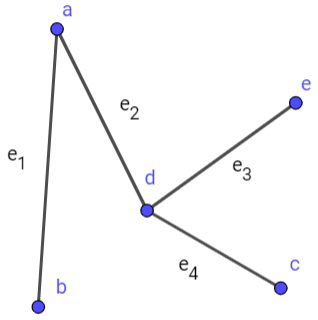
\includegraphics[width = 0.35\linewidth]{./images/graph_definition.png}
    \caption{图 $ G = (V, E, \psi) $}
\end{figure}

\paragraph{例}
上图 $ G $, 其顶点集 $ V = \set{a, b, c, d, e} $, 边集 $ E = \set{e_1, e_2, e_3, e_4} $. 而边和点之间的对应关系为:
\[ \begin{array}{c}
    \psi(e_1) = (a, b) \,,\\
    \psi(e_2) = (a, d) \,,\\
    \psi(e_3) = (d, e) \,,\\
    \psi(e_4) = (d, c)
\end{array} \,.\]

下面概念描述了由原图得到其它图的方法.
\begin{definition}[\text{子图}]
    设图 $ G = (V, E) $, $ V' \subseteq V $, $ E' \subseteq E $, 则图 $ G' = (V', E') $ 称为 $ G $ 的子图. 若 $ G' \neq G $, 则称 $ G' $ 为 $ G $ 的真子图.
\end{definition}

相比子图, 导出子图的概念更常见.

\begin{definition}[\text{点导出子图}]
    设 $ G = (V, E) $, $ V' \subseteq V $. 定义 $ V' $ 的点导出子图 (vertex-induced subgraph) 为 $ G(V') = (V', E') $, 其中:
    \[ E' \coloneqq \set{(a, b) \in E \mid a, b \in V'} \,.\]
\end{definition}

换句话说, $ G(V') $ 的边集由 $ E $ 中关联 $ V' $ 中任意顶点的的边构成. 这意味着两方面: (1) $ V' $ 中任意两点若在 $ G $ 中关联, 则这条边就在导出子图中; (2) 若 $ (a, b) $ 为导出子图中的一条边, 则 $ a, b $ 在原图中也是关联的.

同理还可得到边导出子图.

\begin{definition}[\text{删除点}]
    对于图 $ G = (V, E) $, 设 $ v \in V $. 则删掉这个点及其关联的边, 剩下的图记作 $ G - v $. 也即:
    \[ \begin{cases}
        V(G - v) \coloneqq V - \set{v} \\
        E(G - v) \coloneqq \set{(a, b) \in E \mid a \neq v \land b \neq v} 
    \end{cases} \,.\]

    注意: $ E(G - v) $ 的等价定义为 $ \set{(a, b) \in E \mid a, b \in V - \set{v}} $.
    \vskip 1em
    同理还可以得到删除多个点及其中每个点关联的边得到的图, 记点集 $ V' \subseteq V $. 则 $ G - V' $ 可以定义为:
    \[ \begin{cases}
        V(G - V') \coloneqq V - V' \\
        E(G - V') \coloneqq \set{(a, b) \in E \mid a, b \in V - V'} 
    \end{cases} \,.\]
\end{definition}

从导出子图以及删点子图的定义, 不难得到下面的结论:
\begin{proposition}
    设 $ G = (V, E) $, 若 $ V' $ 和 $ V'' $ 为 $ V $ 的一个划分, 即: $ V' \cap V'' = \varnothing $ 且 $ V' \cup V'' = V $. 则有:
    \[ G(V') = V - V'' \,,\]
    \[ G(V'') = V - V' \,.\]
\end{proposition}

也就是说, 导出子图 $ G(V') $ 可以定义为删去所有除 $ V' $ 之外的点 (即 $ V'' $) 以及其关联的边后剩下的图.

\subsection{点度}
\begin{definition}[\text{度}]
    无向图中, 点 $ v $ 的度数定义为与这个点相关联的边的数目, 记作 $ d(v) $ 或 $ \deg(v) $. 有向图中, 点 $ v $ 的度分为出度和入度: 出度为以 $ v $ 为起点的边的数目, 记作 $ d^+(v) $; 入度为以 $ v $ 为终点的边的数目, 记作 $ d^-(v) $.
\end{definition}

\begin{remark}
    出度为正, 入度为负的规定方式和散度的正负类似.
\end{remark}

\begin{theorem}[\text{握手定理}]
    无向图 $ G = (V, E) $ 满足所有点度之和等于边数量的两倍:
    \[ \sum_{v \in V} d (v) = 2 |E| = 2 \varepsilon(G) \,.\]

    而在有向图中, 有类似的关系:
    \[ \sum_{v \in V} d^+(v) = \sum_{v \in V} d^-(v) =  \varepsilon(G) \,.\]
\end{theorem}

由握手定理可以得到下面的推论 (为引述方便, 称度数为奇数的点为奇点, 度数为偶数的点为偶点):
\begin{proposition}
    对于任意无向图, 奇点的个数一定为偶数.
\end{proposition}



\section{连通性}
\begin{definition}[\text{道路, 简单道路与路径}]
    定义道路 (walk) 为一系列交替的点和边的序列: $ v_0, e_1, v_1, e_2, v_2, \dots, e_n, v_n $; 其中 $ e_i $ 关联 $ v_{i - 1} $ 和 $ v_i $. 
    \begin{itemize}
        \item 若道路中除首尾两个点, 没有相同的节点, 即对任意 $ 1 \leqslant i, j \leqslant n - 1 $, 有 $ v_i \neq v_j $, 则称该道路为简单道路 (path)
        \item 若道路中没有重复的边, 则称其为路径 (trail)
        \item 若道路首尾两点为同一点, 则称其为回路; 若简单道路的首位两点为同一点, 则称其为简单回路
    \end{itemize}
\end{definition}

对于道路 $ v_0, e_1, v_1, \dots, v_{n - 1}, e_n, v_n $, 其含有 $ n $ 条边, 称这条道路的长度为 $ n $, 记作 $ d(v_0, v_n) = n $.

下面几张示意图描述了上面几个术语之间的区别, 注意箭头并不表示有向图, 数字也不代表赋权, 此处只是形象化的表示出这条道路从起点到终点的行进过程和顺序.
\begin{figure}[H]
    \centering
    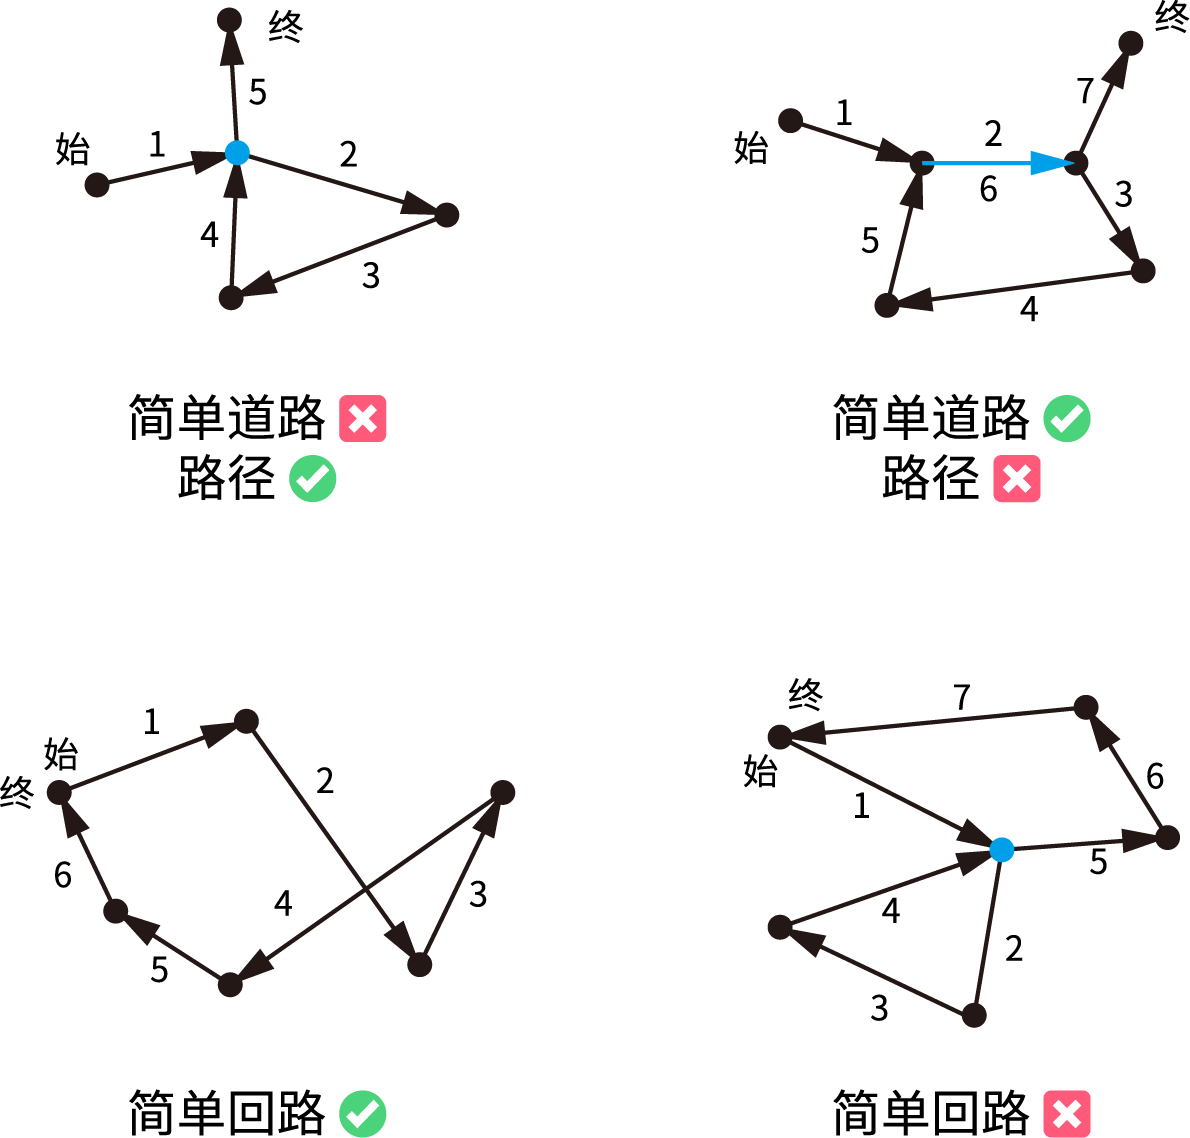
\includegraphics[width = 0.7\linewidth]{./images/path_trail.png}
\end{figure}


\begin{definition}[\text{连通分支}]
    设 $ G $ 为无向图, 则 $ G $ 的一个连通分支是 $ G $ 的一个子图 $ G' $, 且 $ G' $ 不是另一连通分支的子图. 换句话说, $ G $ 的连通分支是 $ G $ 的一个极大连通子图. 图 $ G $ 连通分支的个数记作为 $ \omega(G) $.
\end{definition}

\paragraph{例}
下图用红蓝橙三种颜色标注出了三个连通分支, 该图的连通分支数 $ \omega(G) = 3 $:
\begin{figure}[H]
    \centering
    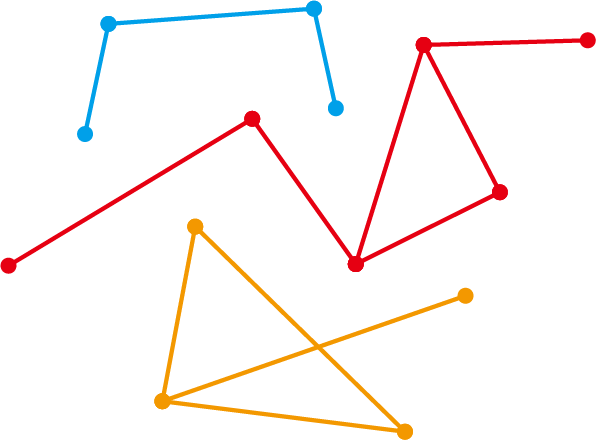
\includegraphics[width = 0.3\linewidth]{./images/branch.png}
\end{figure}



\subsection{连通度}
\begin{definition}[\text{点割集/割点}]
    设 $ G = (V, E) $ 为无向连通图, $ V' \subseteq V $. 若删去 $ V' $ 后, $ G - V' $ 不再连通, 则称 $ V' $ 为 $ G $ 的一个点割集. 若 $ V' $ 是单元素集, 则这个点 $ v $ 称为割点.
\end{definition}

\begin{definition}[\text{边割集/割边}]
    设 $ G = (V, E) $ 为无向连通图, $ E' \subseteq E $. 若删去 $ E' $ 后, $ G - E' $ 不再连通, 则称 $ E' $ 为 $ G $ 的一个边割集. 若 $ V' $ 是单元素集, 则这个边 $ e $ 称为割边或桥.
\end{definition}

\paragraph{例}
下图中, 删除蓝色的点, 原本的连通图变得不再连通, 所以这个点为割点. 删除红色的边, 图也变得不连通, 所以这条边为割边(或桥).
\begin{figure}[H]
    \centering
    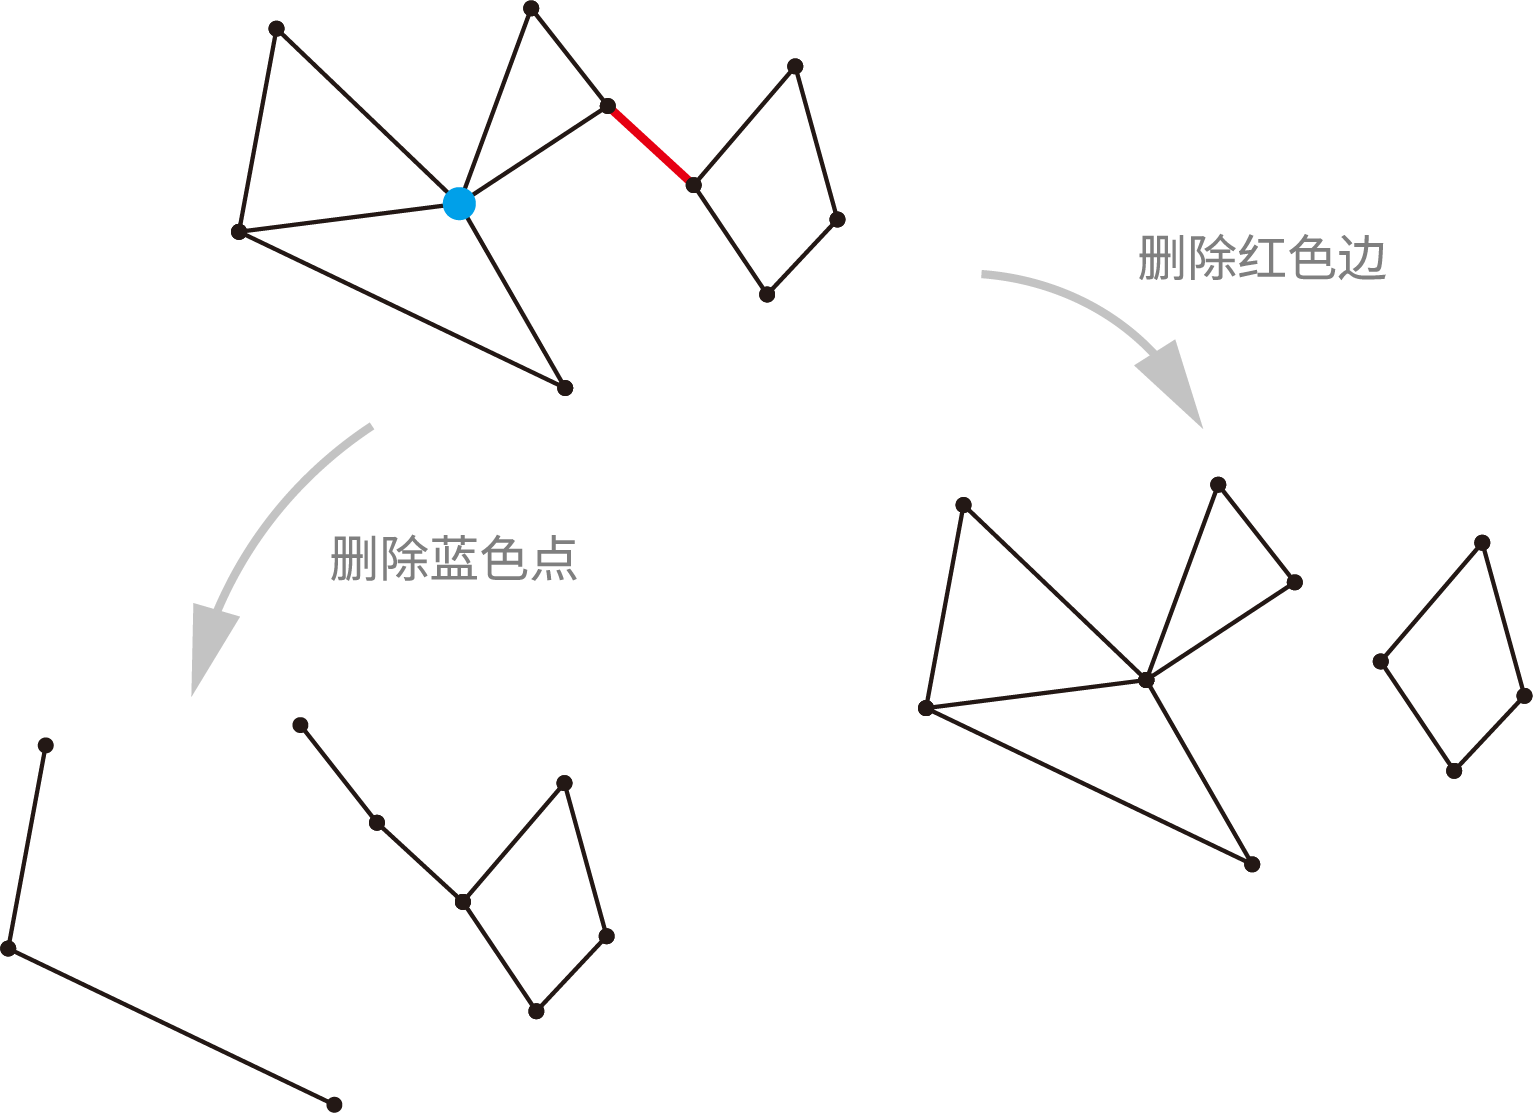
\includegraphics[width = 0.7\linewidth]{./images/bridge.png}
\end{figure}


\begin{definition}[\text{连通度}]
    设 $ G $ 的点割集族为 $ \set{V_1, V_2, \dots, V_n} $, 则定义点连通度(简称连通度)为:
    \[ \kappa(G) \coloneqq \min\set{|V_1|, |V_2|, \dots, |V_n|} \,,\]

    即最小的点割集基数. 同理可以定义边连通度 $ \lambda(G) $.
\end{definition}

换句话说, 点/边连通度描述了使图不再连通需要删除的最少的点/边的数量. 容易得到, 对于 $ n $ 个点 $ 0 \leqslant \kappa(G) \leqslant n - 1 $, $ 0 \leqslant \lambda(G) \leqslant n - 1 $. 而如果 $ G $ 本就是不连通的, 则定义 $ \kappa(G) = \lambda(G) = 0 $, 因为无需删点/边就能达到不连通. $ n $ 个顶点的图, 连通度不能为 $ n $, 因为删去所有顶点没有意义.

注意到一点, 对于完全图 $ K_n $, 无论删去多少点, 图总是连通的, 所以定义 $ K_n $ 的点连通度和边连通度 $ \kappa(K_n) = \lambda(K_n) = n - 1 $, 后面会说明, $ n $ 阶非完全图的最大连通度只能大到 $ n - 2 $, 所以剩下的 $ n - 1 $ 分配给完全图是很自然的.

综上所述, 可以通过给定点连通度, 图有两种情况:
\begin{itemize}
    \item 点连通度为 $ 0 $: $ G $ 不连通或 $ G $ 只有一个顶点 (即 $ K_1 $)
    \item 点连通度为 $ 1 $: $ G $ 最少删去 $ 1 $ 个顶点就不再连通, 或 $ G $ 为完全图 $ K_2 $
    \item 点连通度为 $ n $: $ G $ 最少删去 $ n $ 个顶点就不在连通, 或 $ G $ 为完全图 $ K_{n + 1} $
\end{itemize}

\paragraph{例}



\begin{proposition}
    无向图中, 下面三个命题等价:
    \begin{itemize}
        \item $ \kappa(G) = n - 1 $
        \item $ \lambda(G) = n - 1 $
        \item $ G $ 是完全图 $ K_n $
    \end{itemize}
    也就是说: 若 $ n $ 顶点图 $ G $ 不是完全图, 则 $ \kappa(G) \leqslant n - 2 $, $ \lambda(G) \leqslant n - 2 $.
\end{proposition}

\begin{proposition}
    设有无向图 $ G $, 其点连通度 $ \kappa(G) $, 边连通度 $ \lambda(G) $ 和最小点度 $ \delta(G) $ 存在不等关系:
    \[ \kappa(G) \leqslant \lambda(G) \leqslant \delta(G) \,.\]
\end{proposition}





\end{document}